\documentclass{article} 

\usepackage{graphicx}

\usepackage{mdframed}
\usepackage{listings,lstautogobble}
\usepackage{hyperref}
\usepackage{amsfonts}
\usepackage{amsmath}

\graphicspath{img}

\title{CSE160 Homework 3}
\author{Elijah Hantman}

%\renewcommand{\spn}[1]{\langle #1 \rangle}

\setlength{\emergencystretch}{10pt}

\begin{document}
    \maketitle

    {\large Colors}
    \begin{enumerate}
        \item Fill in the blanks below to convert colors
            between RGB, HSV, and CMY models:

            \begin{table}[h]
                \resizebox{\textwidth}{!}{
                \begin{tabular}{|c c c|c c c|c c c|}
                    \hline
                    Red & Green & Blue & Hue & Saturation & Value & Cyan & Magenta & Yellow\\
                    \hline
                    0 & 0 & 0 & 0 & 0 & 0 & 1 & 1 & 1\\  
                    255 & 255 & 0 & 60 & 100 & 100 & 1 & 1 & 0\\
                    0 & 0 & 127.5 & 240 & 100 & 50 & 1 & 1 & 0\\
                    255 & 255 & 255 & 0 & 0 & 100 & 0 & 0 & 0\\
                    0 & 255 & 255 & 180 & 100 & 100 & 1 & 0 & 0\\
                    255 & 0 & 0 & 0 & 100 & 100 & 0 & 1 & 1\\
                    255 & 255 & 255 & 180 & 0 & 100 & 0 & 0 & 0\\
                    0 & 0 & 0 & 300 & 50 & 0 & 1 & 1 & 1\\
                    \hline
                \end{tabular}
            }
            \end{table}

        \item Given a color $c_1 = RGB(25,127,76)$, which color $c_2$ can you add to get a color pink?
            Define (using the RGB model) the pink you are aiming and then the color you
            added.

            \begin{mdframed}
                Assuming pink would be something like $RGB(255, 0, 100)$. 

                Then I need $c_2 = RGB(255 - 25, 0 - 127, 100 - 76)$.
                Giving $c_2 = RGB(230, -127, 34)$. Of course this is not
                a valid color meaning that we can't additively blend to
                this color.

                We could pick some mixture of this color and white however,
                to do this we add $127$ to each component to get
                $c_2 = RGB(255, 0, 161)$. This will give the same hue
                but a lighter shade.
            \end{mdframed}

            \break
        \item Sketch the color models for RGB (cube) and HSV (cone). In both model sketches,
            mark (with color name) the position of each of the following colors: black, white,
            gray, red, cyan, and yellow

            \begin{figure}[h]
            \begin{center}
                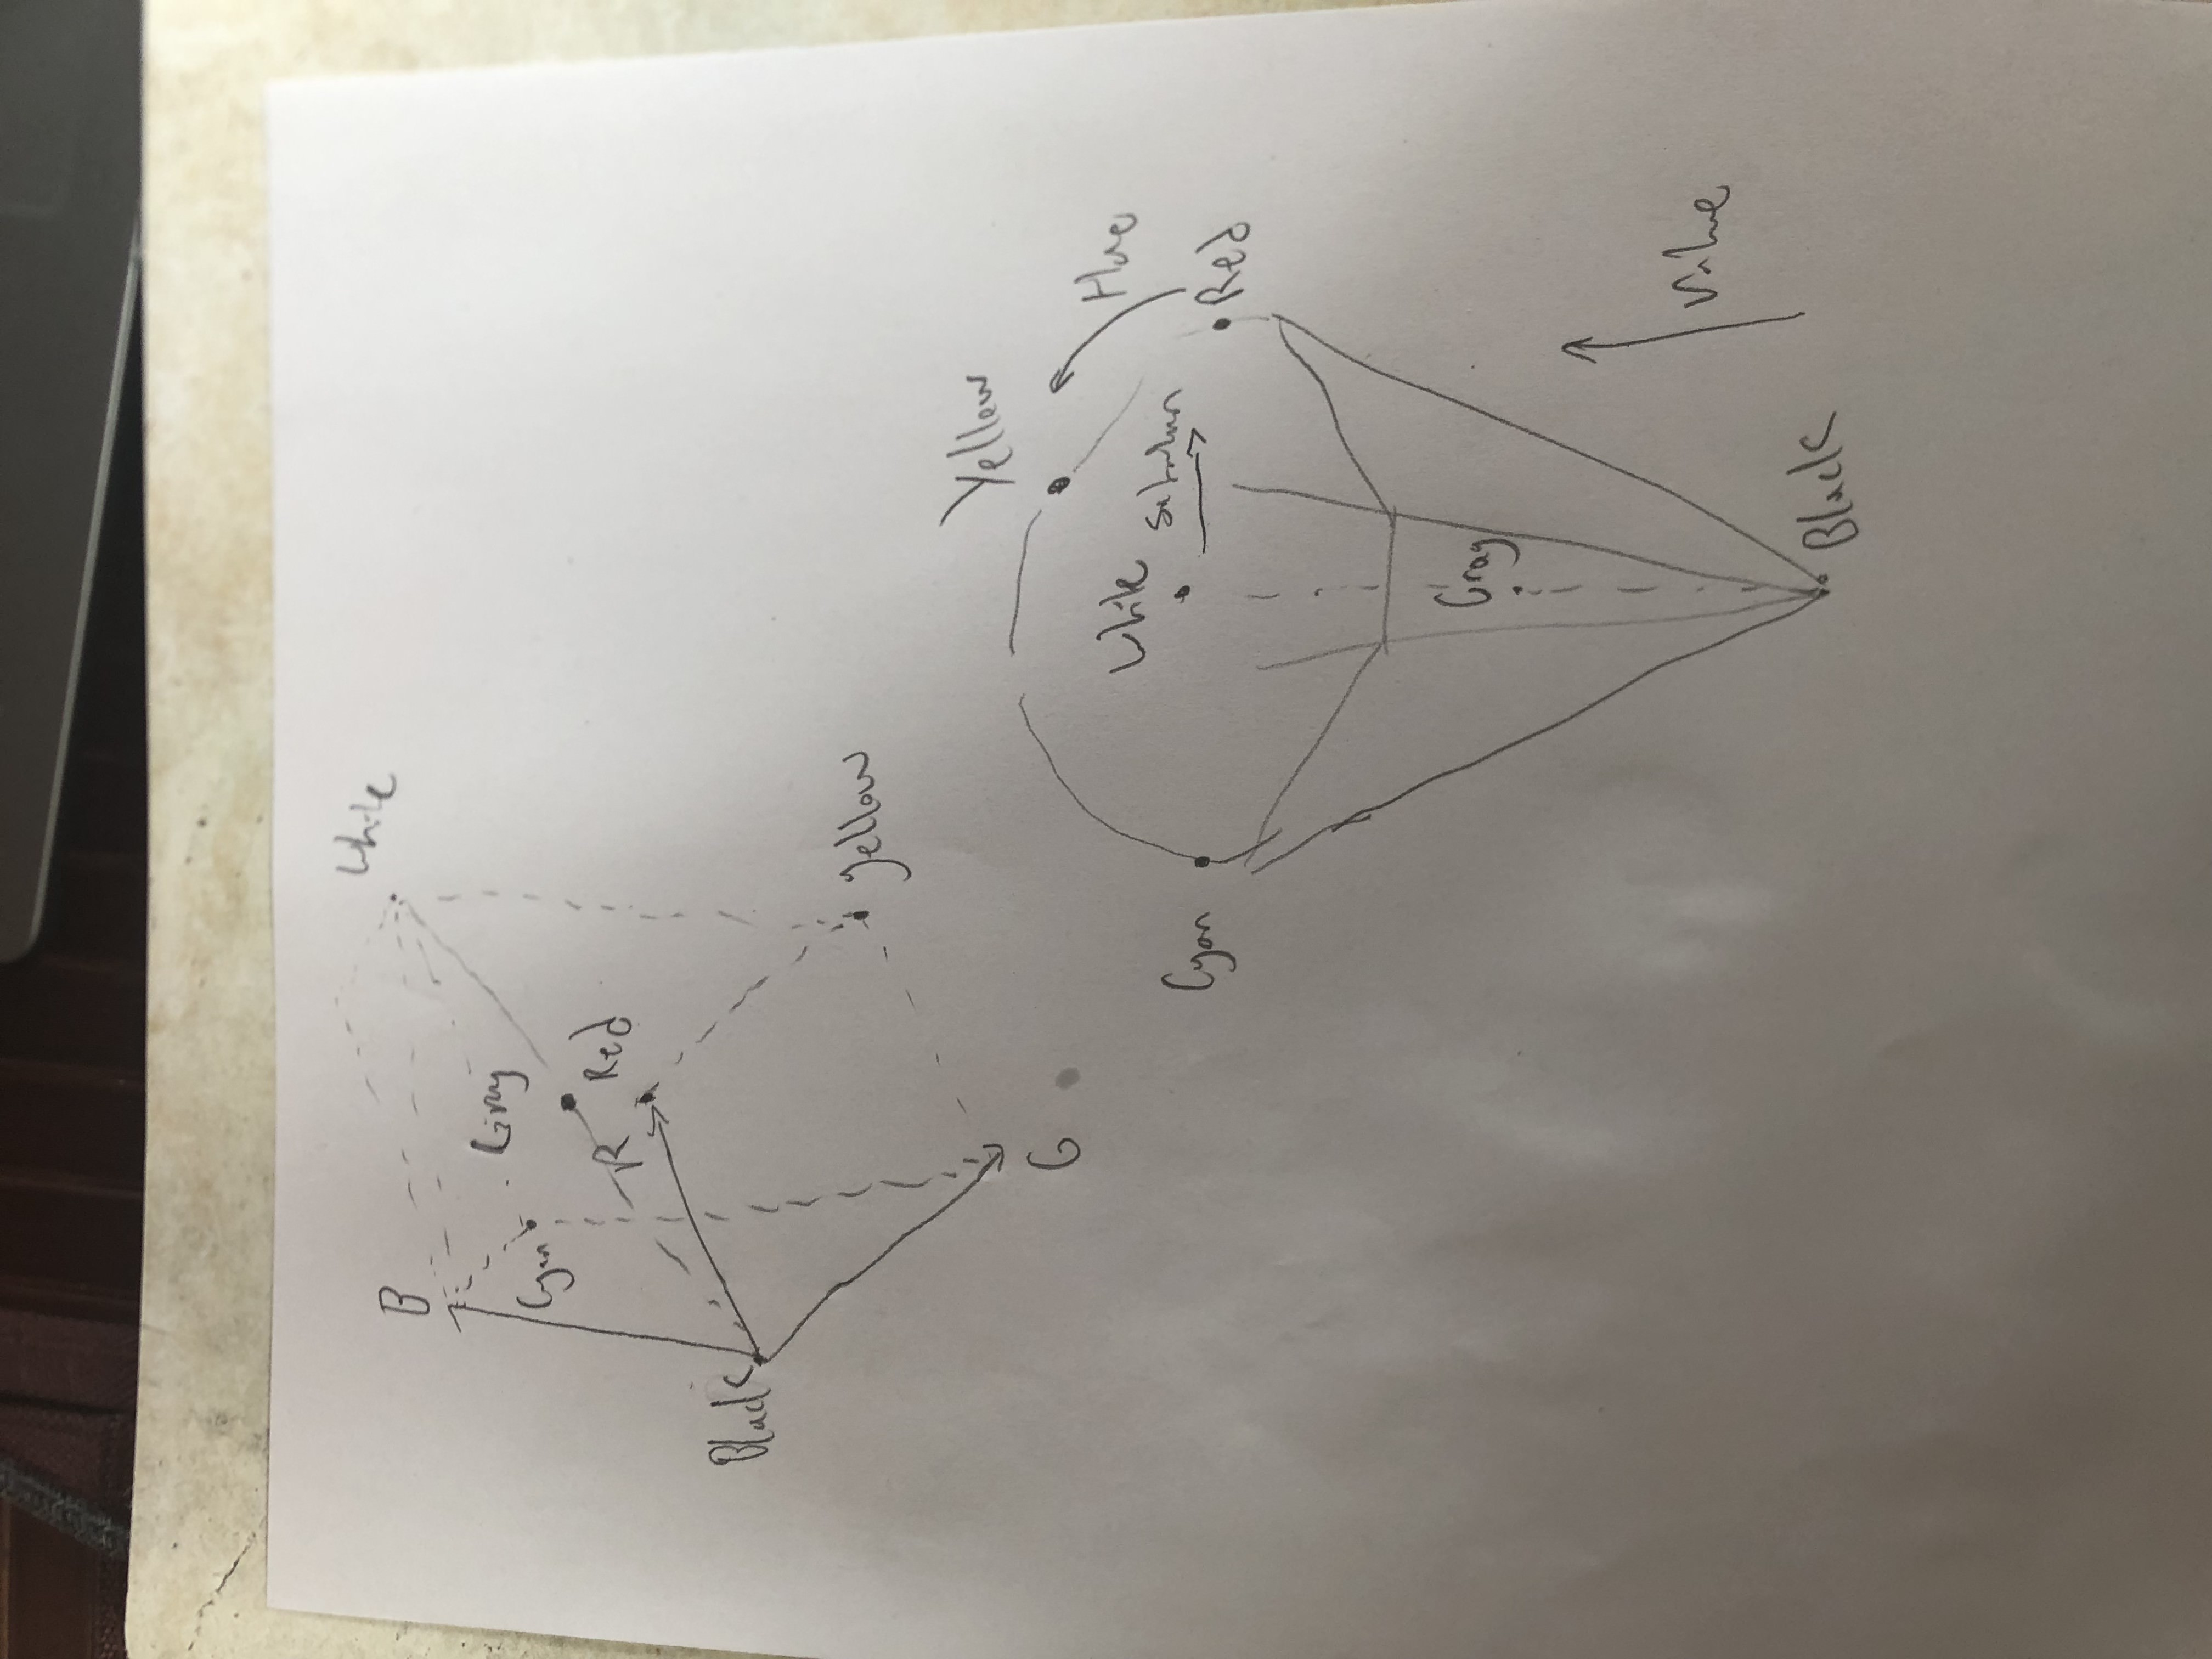
\includegraphics[scale=0.07, angle = -90]{img/Colormodel.jpg}
            \end{center}
            \end{figure}

        \item Given the color $c_1 = RGB(255,255,0)$, if you decrease the ”saturation” as defined
            in HSV until fully desaturated, describe the range of RGB colors you will pass
            through, as well as the final result.
            
            \begin{mdframed}
                The initial color is a maximally bright Yellow. As the saturation is decreased the yellow
                will be blended with more and more white until the color is pure white.
            \end{mdframed}

        \item Linearly interpolate the color halfway between red and blue in each of the following
            color models. (Requires a separate calculation for each subproblem, not just
            converting the resulting color.)
            \begin{enumerate}
                \item RGB

                    \begin{mdframed}
                        The color which is red is $r = RGB(255, 0, 0)$.
                        And the color blue is $b = RGB(0, 0, 255)$.

                        To blend we do $0.5r + 0.5b$.

                        \begin{displaymath}
                            0.5r + 0.5b =
                            RGB(127.5, 0, 125.5)
                        \end{displaymath}

                        This is a slightly dark purple.
                    \end{mdframed}

                \item HSV

                    \begin{mdframed}
                        In HSV

                        $r = HSV(0, 100, 100)$
                        and $b = HSV(240, 100, 100)$.

                        Same formula as before:

                        \begin{displaymath}
                            0.5r + 0.5b = 
                            HSV(120, 100, 100)
                        \end{displaymath}

                        This is a bright green.
                    \end{mdframed}
                \item CMY
                    \begin{mdframed}
                       \begin{displaymath}
                           r = CMY(0, 1, 1)
                       \end{displaymath} 
                       \begin{displaymath}
                           b = CMY(1, 1, 0)
                       \end{displaymath}

                       Then we blend:

                       \begin{displaymath}
                           0.5r + 0.5b =
                           CMY(0.5, 1, 0.5)
                       \end{displaymath}

                       Which is a dark purple. We can actually see that
                       this is identical to the color produced in RGB,
                       which makes sense since CMY is an inversion of
                       RGB.
                    \end{mdframed}
                \item Considering the results of Question 5. What can be concluded about linear interpolation
                    in different color spaces?
                    \begin{mdframed}
                        We can see that not all color spaces
                        produce idential results when interpolating.

                        However, I believe that color spaces
                        which are linear relative to each other
                        do produce the same colors. The reason is that
                        if the transformation from one color space to
                        another is linear then it has the following properties.

                        \begin{displaymath}
                            f(a + b) = f(a) + f(b)
                        \end{displaymath}
                        \begin{displaymath}
                            f(\lambda a) = \lambda f(a)
                        \end{displaymath}

                        These properties mean that we can extract the linear transformation
                        from the linear interpolation equation.

                        However, HSV is not a linear mapping of RGB, which is
                        why it produces different outputs.
                    \end{mdframed}

            \end{enumerate}
        \item Consider the following javascript snippet to setup a vertex buffer and the the pair
            of vertex/fragment shaders defined in GLSL:

            {
                \begin{figure}[h]
                    \hfuzz=50pt
                    \begin{lstlisting}[language=C, gobble=24]
                        // === VERTEX SHADER
                        attribute vec2 a_Position;
                        attribute vec3 a_Color;
                        varying vec3 v_Color;
                        main() {
                            v_Color = a_Color;
                            1
                            gl_Position = vec4(a_Position, 0.0, 1.0);
                        }
                        // === FRAGMENT SHADER
                        varying vec3 v_Color;
                        main() {
                            gl_FragColor = vec4(v_Color, 1.0);
                        }
                        // === VERTEX BUFFER SETUP IN JAVASCRIPT
                        gl.clearColor(0.0, 0.0, 0.0, 1.0);
                        gl.clear(gl.COLOR_BUFFER_BIT);
                        let vertices = new float32array([ __ ]);
                        let a_position = gl.getattriblocation(gl.program, "a_position");
                        gl.vertexattribpointer(a_position, __, gl.float, false, __, __ );
                        gl.enablevertexattribarray(a_position);
                        let a_color = gl.getattriblocation(gl.program, "a_color");
                        gl.vertexattribpointer(a_color, __, gl.float, false, __, __ );
                        gl.enablevertexattribarray(a_color);
                        gl.bufferdata(gl.array_buffer, vertices, gl.static_draw);
                        gl.drawarrays(gl.triangles, 0, __ );
                    \end{lstlisting}
                \end{figure}
            }
            For each image fill in the blanks which would produce the
            output image.


            \begin{enumerate}
                \item The blanks are listed in order
                    \begin{mdframed}
                       Vertices are 
                       \begin{gather}
                           -1, -1, 1, 0, 0\\ 
                           1, -1, 1, 0, 0\\
                           0, 1, 1, 0, 0
                       \end{gather}

                       With attribs $2, 20, 0$
                       And $3, 20, 8$.

                       Finally there are 3 verts so
                       $3$ is the last blank.
                    \end{mdframed}
                \item The blanks are listed in order
                    \begin{mdframed}
                       Vertices are 
                       \begin{gather}
                           -1, -1, 0, 1, 0\\ 
                           1, -1, 0, 0, 1\\
                           0, 1, 1, 0, 0
                       \end{gather}

                       With attribs $2, 20, 0$
                       And $3, 20, 8$.

                       Finally there are 3 verts so
                       $3$ is the last blank.
                    \end{mdframed}
                \item The blanks are listed in order
                    \begin{mdframed}
                       Vertices are 
                       \begin{gather}
                           -1, -1, 0, 0, 0\\ 
                           1, -1, 0, 0, 0\\
                           0, 1, 0, 1, 0\\
                            \\
                           -1, 1, 0, 1, 0\\ 
                           1, 1, 0, 1, 0\\
                           0, -1, 0, 1, 0
                       \end{gather}

                       With attribs $2, 20, 0$
                       And $3, 20, 8$.

                       Finally there are 6 verts so
                       $6$ is the last blank.
                    \end{mdframed}
                \break
                \item The blanks are listed in order
                    \begin{mdframed}
                       Vertices are 
                       \begin{gather}
                           -1 -1, 0, 0, 0\\
                           1, -1, 0, 0, 1\\
                           -1, 1, 0, 0, 0\\
                           \\
                           1, 1, 0, 0, 1\\
                           -1, 1, 0, 0, 0\\
                           1, -1, 0, 0, 1
                       \end{gather}

                       With attribs $2, 20, 0$
                       And $3, 20, 8$.

                       Finally there are 6 verts so
                       $6$ is the last blank.
                    \end{mdframed}
            \end{enumerate}
    \end{enumerate}

    \break
    {\large Texture}

    \begin{enumerate}
        \item Considering the following chessboard texture with (u,v) coordinates:
            \begin{enumerate}
                \item Draw the approximate mappings if they were
                    textured as follows:
                    \begin{figure}[ht]
                        \begin{center}
                            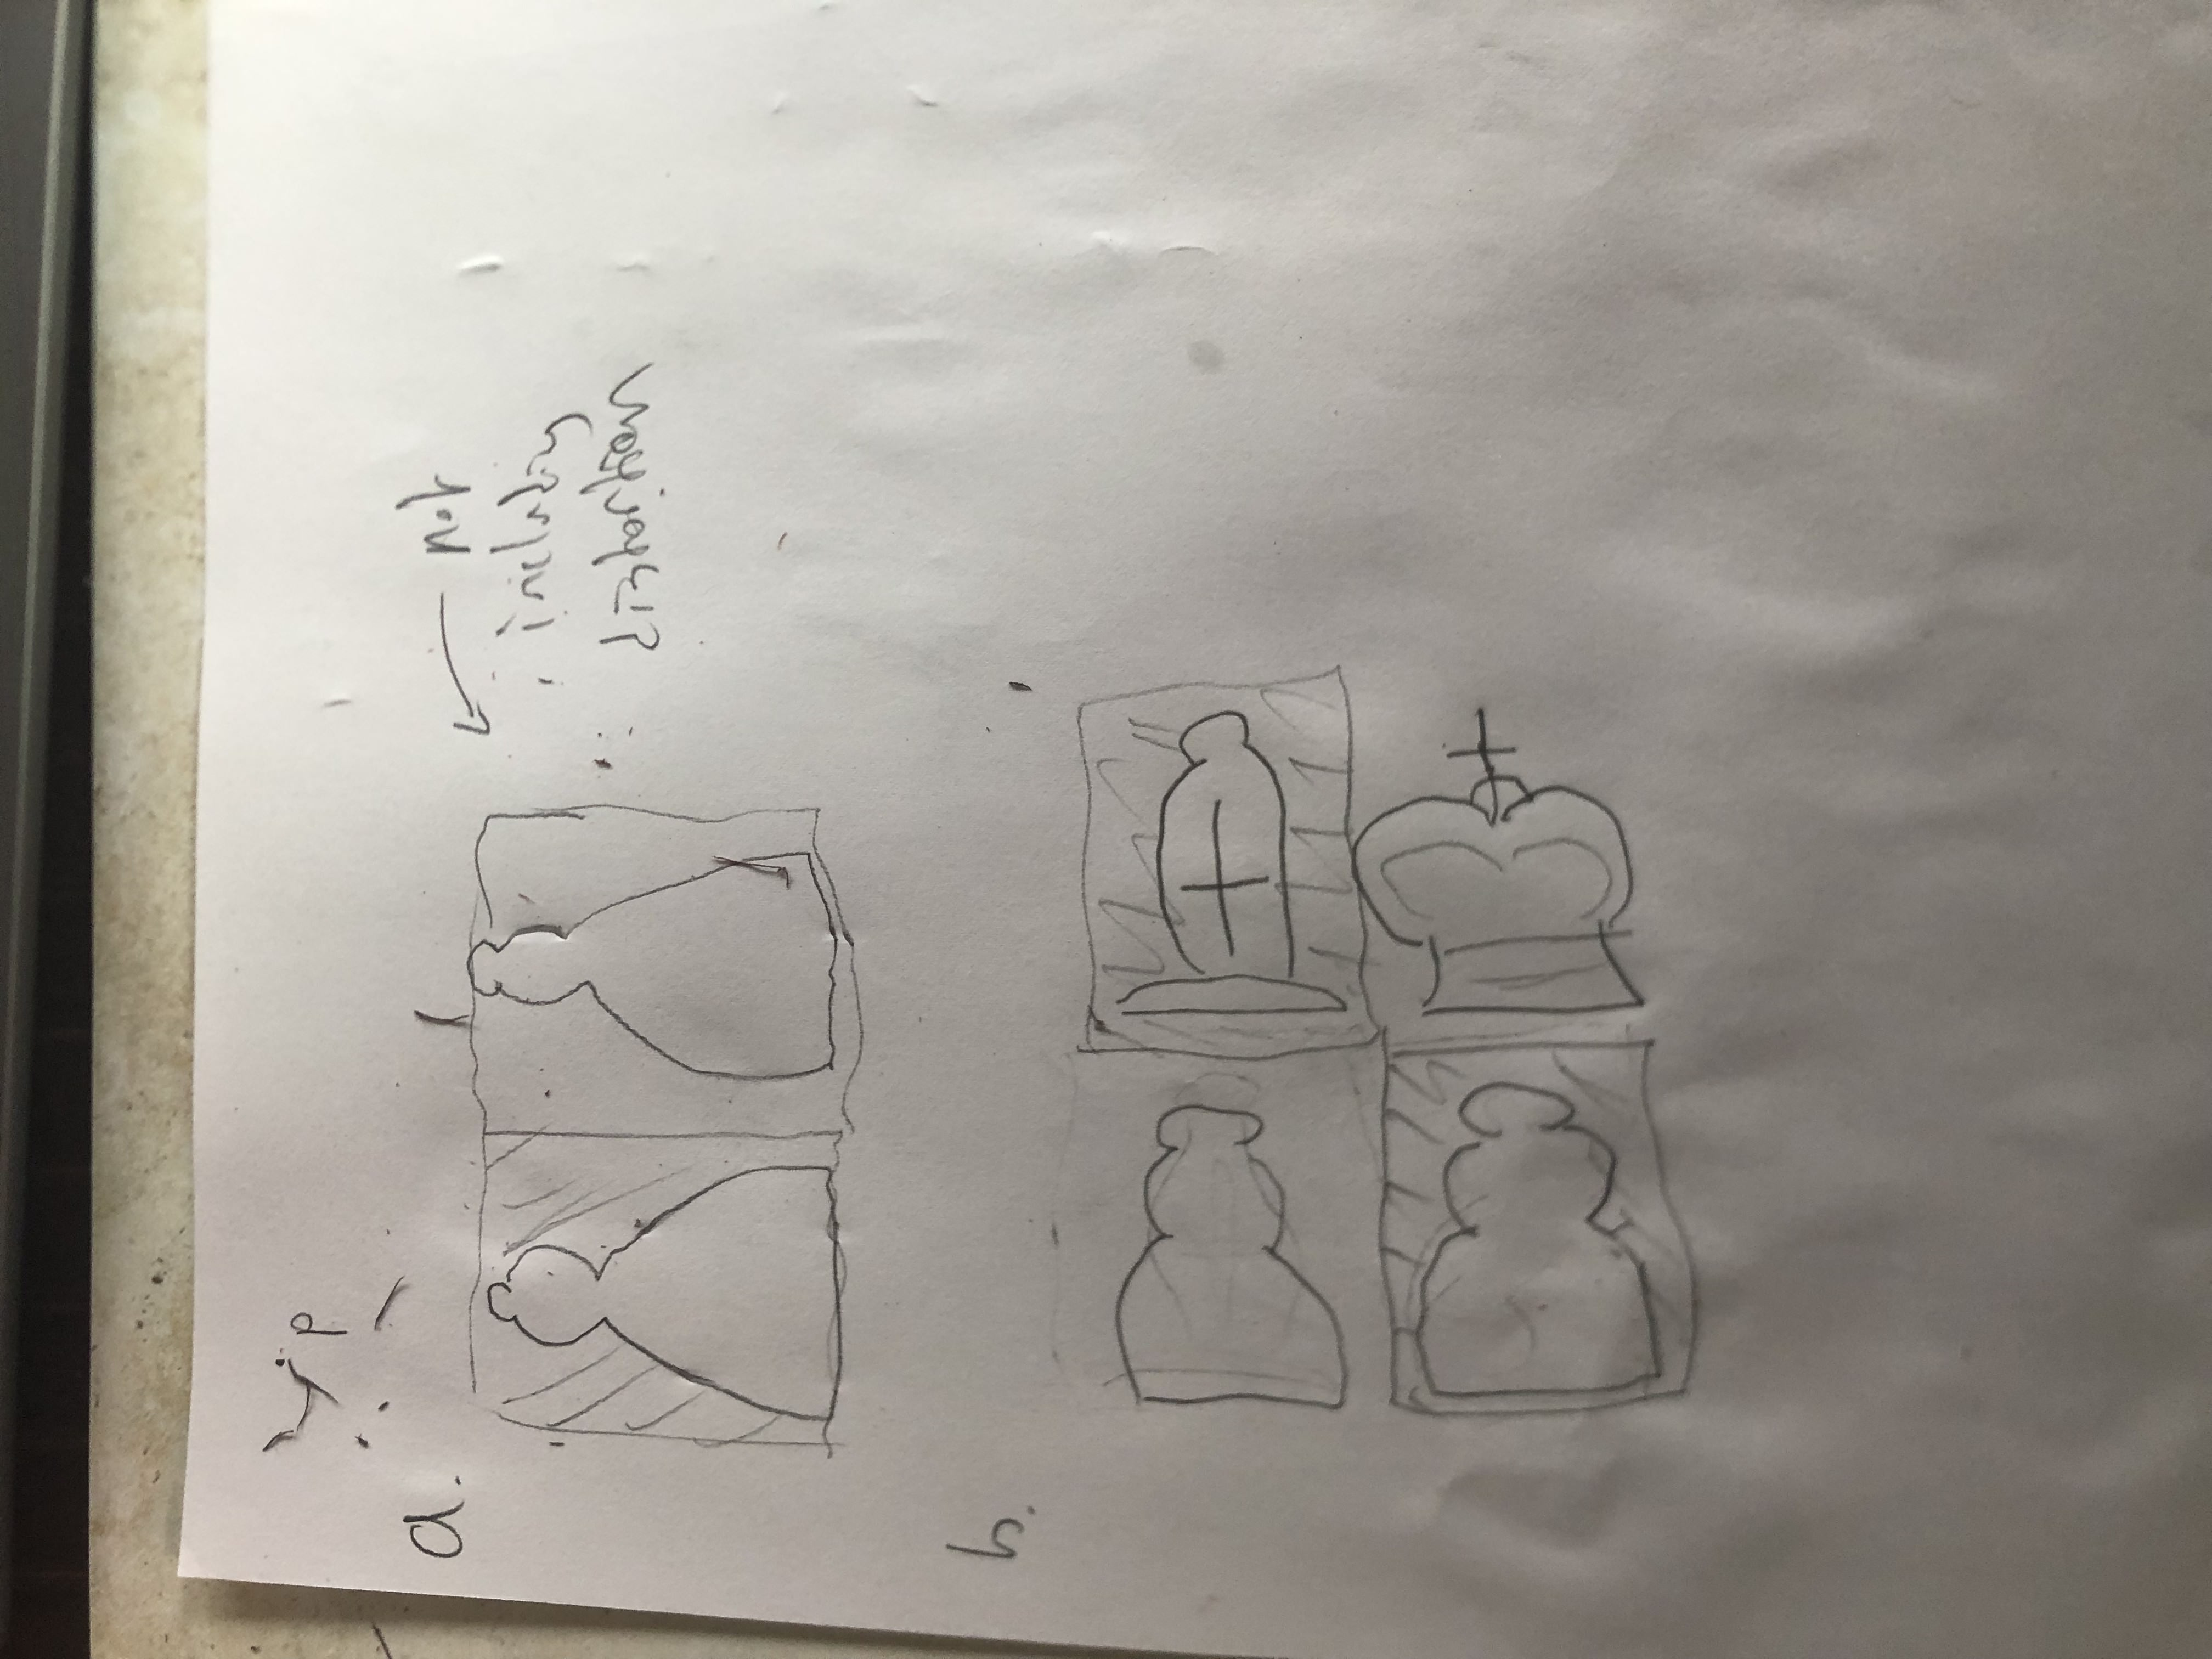
\includegraphics[scale=0.07, angle = -90]{img/uv.jpg}
                        \end{center}
                    \end{figure}
                \item Label the (u,v) coordinates for each of
                    the four vertices of the following images.

                    \begin{mdframed}
                        These will be labeled in the order,
                        top left, top right, bottom left, bottom right.

                        First:
                        \begin{gather}
                            (0.375, 1.0), (0.5, 1.0)\\
                            (0.375, 6/8), (0.5, 6/8)
                        \end{gather}

                        Second:
                        \begin{gather}
                            (3/8, 2/8), (5/8, 2/8)\\
                            (3/8, 0), (5/8, 0)
                        \end{gather}

                        Third:
                        \begin{gather}
                            (1.0, 2/8), (1.0, 0)\\
                            (6/8, 2/8), (6/8, 0)
                        \end{gather}
                    \end{mdframed}
            \end{enumerate}
        
        \item Describe how and when one could use Spherical Parameterization to map a texture
            onto a 3D model.

            \begin{mdframed}
                You would use spherical parameterization to map
                textures onto spheres, or when doing specific kinds of
                map projections.

                Essentially you take each vertex on the sphere in terms of
                the azimuth and elevation, or just two angles, and the radius.
                For texture mapping you just drop the radius and use the
                two angles as your uv coordinates.

                There are other ways to parameterize a sphere, including
                using another shape like a cube and then projecting
                each point on the cube onto the sphere.
            \end{mdframed}

        \item In texture mapping, what is the difference between magnification and minification?
            \begin{mdframed}
                Magnification is when we try to sample between texels, meaning we have more pixels
                than texels.

                Minification happens when we have more texels than pixels and we sample
                the texels sparsely.
            \end{mdframed}

        \item We textured a floor in our world and wish it looked like the left image, instead we
            got the right image, with speckled Moire patterns in the back and Jaggies in the
            front.

            \begin{enumerate}
                \item Explain why these Moire patterns appear and how to fix them.
                    \begin{mdframed}
                        The patterns appear due to the texel sampling returning the color
                        of the texel exactly and not the average of all the texels the pixel covers.
                        This can be solved via either mipmapping where we do a proper downsample,
                        or via multisampling anti aliasing which will take multiple texel samples and
                        average their values. We can also use anisotropic filtering which changes how
                        the textures are sampled to look better at oblique angles.
                    \end{mdframed}

                \item Explain why these Jaggies patterns appear and how to fix them.
                    \begin{mdframed}
                        The jaggies appear because where the pixel samples the geometry is only in a single
                        spot. So the pixels are either entirely within the lines or they are outside causing the
                        lines to be jagged on the pixel grid. To fix this we want to either use
                        some kind of interpolation for our textures, or you could use an anti-aliasing technique
                        like super sampling. Interpolation tends to give a somewhat blurry look so you could also
                        use an SDF with a threshhold alongside something like MSAA, which would preserve
                        the sharp lines and the MSAA would help reduce the aliasing so you can have both without
                        blurring.
                    \end{mdframed}
            \end{enumerate}

        \item What is the following fragment shader doing?
            \begin{lstlisting}[language=C,gobble = 16]
                varying vec2 uv;
                uniform sampler2D tex;
                uniform vec4 baseColor;
                void main() {
                    vec4 texColor = texture2D(tex, uv);
                    gl_FragColor = 0.5 * texColor + 0.5 * baseColor;
                } 
            \end{lstlisting}

            \begin{mdframed}
                It looks like the shader is sampling a texture
                according to uv coordinates passed via the vertex shader,
                then it is blending it with a base color passed via the uniform.

                The blend uses an equal weight of the texture and base color, giving
                the effect of mixing the texture with a static color.
            \end{mdframed}
    \end{enumerate}


    {\large Readings}
    \begin{enumerate}
        \item What is the difference between using multiple buffers to store vertex data vs. interleaving vertex
            data in one buffer?
            \begin{mdframed}
                The main difference is data layout. With multiple buffers you can
                swap out just the attributes, and if you are storing the attributes separately on
                the cpu anyways, say for example you have a model and you store the uv and positions of
                the vertices in separate buffers, then it can be very direct to use multiple buffers.

                However, the textbook recommends interleaving, which uses a single buffer. This does
                mean fewer buffers, and if you are using something like gl.bufferSubData, then it
                might make managing the lengths of each buffer easier.

                Of course there are also alignment concerns, it is possible that the driver may have to do
                more work if your data is not packed to specific byte boundaries and multiple buffers may be
                used to reduce this problem. Multiple buffers also make possible vertex pulling which allows
                for huge reductions in the memory footprint of each vertex.
            \end{mdframed}

        \item Describe the two process that take place between the vertex and fragment shaders.
            \begin{mdframed}
                Immediately after the vertex shader is shape assembly, this is where vertices are assembled into primitives
                for the rasterizer. 

                After Assembly there is a tesselation shader, this allows for subdividing geometry and generating new vertices.

                There is also a programmable shader stage following this one called the geometry shader,
                where you can operate directly on geometry, either culling it or generating new geometry.

                Finally there is rasterization, which happens before the fragment shader runs. This is where primitives
                are converted into I believe pixels, which the fragment shader then runs on. The fragment shader actually
                runs on quads and then discards the pixels outside of the geometry.
            \end{mdframed}

        \item In the context of the fragment shader, describe how varying variables can be used to interpolate
            data among fragments

            \begin{mdframed}
                Varying variables are passed in from the vertex shader. During rasterization the data in these variables
                are interpolated between vertices for each fragment. The interpolation is controlled by the position of
                each fragment. In practice you can pass things which you want to smoothly vary across a triangle in,
                and the fragment shader can use it to compute gradients across space, ie: texturing, noise, etc.
            \end{mdframed}

        \item In the context of texture mapping, what is a magnification method? Enumerate and explain
            different methods.

            \begin{mdframed}
                The maginification method is what the texture sampler will use to interpolate when the sample point
                lies between texels. This happens when the texels are larger than individual pixels meaning pixels may lie
                between texels and need to generate new data.

                The values in the text are
                \begin{enumerate}
                    \item LINEAR
                        
                        This uses linear interpolation to blend between 4 pixels, also called
                        Bilinear filtering.

                    \item Nearest

                        This simply uses the nearest texel, usually used in pixel art.
                \end{enumerate}
            \end{mdframed}
        \item In the context of texture mapping, what is a minification method? Enumerate and explain
            different methods.

            \begin{mdframed}
                Minification is when each pixel spans multiple texels. Without filtering this can result in noise,
                moire patterns and other artifacts.

                There are two independent ways to sample.
                First are the two methods that also apply to the mag filters,
                this allows pixels whose sample point falls between texels to blend them.

                Then there is the mipmap usage. Often applications will generate explicit downsampled
                versions of each image called Mipmaps. These will average the color of each
                pixel so that it looks more natural. You can either use the nearest mipmap level,
                or linearly blend between mipmap levels which is called trilinear filtering.
            \end{mdframed}
    \end{enumerate}

\end{document}
